\documentclass[conference]{IEEEtran}
\IEEEoverridecommandlockouts
% The preceding line is only needed to identify funding in the first footnote. If that is unneeded, please comment it out.

% ============================================
% PACKAGES
% ============================================
\usepackage{cite}
\usepackage{amsmath,amssymb,amsfonts}
\usepackage{algorithmic}
\usepackage{graphicx}
\usepackage{textcomp}
\usepackage{xcolor}
\usepackage{booktabs}
\usepackage{hyperref}
\usepackage{enumitem}
\usepackage{tikz}
\usetikzlibrary{shapes.geometric, arrows.meta, positioning, calc}

\def\BibTeX{{\rm B\kern-.05em{\sc i\kern-.025em b}\kern-.08em
    T\kern-.1667em\lower.7ex\hbox{E}\kern-.125emX}}

% ============================================
% DOCUMENT
% ============================================
\begin{document}

\title{Vulnerabilities of Small Language Models: A Systematic Literature Review}

\author{\IEEEauthorblockN{Daniel Dias}
\IEEEauthorblockA{\textit{Department of Informatics Engineering} \\
\textit{Polytechnic School of Porto}\\
Porto, Portugal \\
1240145@isep.ipp.pt}
}

\maketitle

% ============================================
% ABSTRACT
% ============================================
\begin{abstract}
\textbf{Context:} Small Language Models (SLMs), typically defined as transformer-based architectures with fewer than 10 billion parameters, are increasingly deployed in edge computing, mobile applications, and IoT systems where resource constraints preclude larger models. The rapid adoption of SLMs has outpaced systematic investigation of their security properties.
\textbf{Objective:} This systematic literature review identifies, categorizes, and analyzes security vulnerabilities specific to SLMs, examining how these vulnerabilities differ from those in larger models and evaluating the effectiveness of proposed defenses.
\textbf{Methods:} Following PRISMA 2020 guidelines, we searched arXiv, Semantic Scholar, and ACL Anthology, identifying 75 records. After duplicate removal and screening, 65 studies published between 2020 and 2025 were included. Quality assessment classified 37\% as high quality, 49\% as medium, and 14\% as lower quality.
\textbf{Results:} SLMs exhibited significantly higher jailbreak susceptibility than LLMs, with median attack success rates of 34\% compared to 15\% for equivalently aligned larger models. Post-training quantization to 4-bit precision increased jailbreak vulnerability by 25\%. Conversely, SLMs demonstrated reduced privacy attack vulnerability due to lower memorization capacity. Backdoor attacks achieved near-perfect success rates independent of model size. Evaluation of defense mechanisms revealed that eight of ten established defenses were bypassed by adaptive attacks.
\textbf{Conclusions:} SLMs present a distinct security profile requiring dedicated frameworks rather than adapted LLM approaches. The gap between deployment acceleration and security framework maturation represents a critical challenge for edge AI applications.
\end{abstract}

\begin{IEEEkeywords}
Small Language Models, Security Vulnerabilities, Jailbreak Attacks, Backdoor Attacks, Model Quantization, Edge Computing, Systematic Literature Review
\end{IEEEkeywords}

% ============================================
% I. INTRODUCTION
% ============================================
\section{Introduction}

The field of natural language processing has undergone a fundamental transformation with the advent of transformer-based architectures \cite{vaswani2017attention} and the subsequent development of Large Language Models. Systems such as GPT \cite{achiam2024gpt4}, Claude, and Gemini have demonstrated remarkable capabilities in reasoning, code generation, and creative tasks, driven by scaling to hundreds of billions of parameters \cite{brown2020language,zhao2023survey}. These foundation models have reshaped expectations for artificial intelligence and attracted substantial industrial investment \cite{bommasani2021opportunities}.

Yet a critical countertrend is emerging: the rise of small language models designed for practical deployment and mitigating private data leakage. Small language models, typically defined as transformer-based architectures with around 7-10 billion parameters \cite{lu2024slm_survey, belcak2025slm_agentic}, have emerged as compelling alternatives that address fundamental limitations of their larger counterparts. SLMs require substantially less memory and processing power, enabling deployment on hardware ranging from consumer GPUs to mobile devices and IoT systems, with proportionally reduced operational costs \cite{lu2024slm_survey, tang2025demystifying}. Edge deployment enables real-time inference without network latency, critical for autonomous systems, industrial automation, and responsive interfaces. Privacy-sensitive applications benefit from local inference, eliminating the need to transmit confidential data to cloud services. Models such as Microsoft's Phi-2 \cite{phi2}, TinyLlama \cite{tinyllama}, and Google's Gemma \cite{gemma} have demonstrated that compact architectures can achieve remarkable performance on targeted tasks, challenging assumptions about the necessity of scale. Recent work from NVIDIA researchers argues that small language models represent the future of agentic AI systems, as the specialized and repetitive tasks characteristic of such systems are better suited to smaller, more efficient models \cite{belcak2025slm_agentic}. This perspective reflects a broader recognition that practical considerations of cost, latency, and deployment constraints increasingly favor compact alternatives.

However, the rapid adoption of small language models has outpaced systematic investigation of their security properties, creating significant risks for deploying organizations. Zhang et al. found that nearly half of the 63 SLMs they tested exhibited attack success rates exceeding 40\% against jailbreak attempts, while over one-third failed to resist even straightforward harmful requests \cite{zhang2025slm_jailbreak}. The fundamental challenge lies in the tension between model capacity and security implementation: safety mechanisms that function effectively in models with hundreds of billions of parameters may degrade or fail entirely when compressed into smaller architectures \cite{li2025quantized_jailbreak}. Yi et al. documented how compression techniques commonly used to create deployable SLMs can compromise security robustness, revealing ``submerged threats'' that emerge from efficiency optimizations \cite{yi2025slm_submerged}. Edge deployment introduces additional attack surfaces, as models operating in physically accessible environments face threats ranging from adversarial input injection \cite{wang2022adversarial_nlp_survey} to direct model extraction \cite{carlini2024stealing,yao2024survey_extraction}. The combination of reduced defensive capacity and expanded attack surface creates a security landscape that demands dedicated investigation, distinct from the extensive but LLM-focused security literature \cite{xu2024jailbreak_survey}.

% ============================================
% II. METHODOLOGY
% ============================================
\section{Methodology}

This systematic literature review follows the Preferred Reporting Items for Systematic Reviews and Meta-Analyses (PRISMA) 2020 guidelines \cite{page2021prisma} and adopts established protocols for conducting systematic reviews in software engineering \cite{kitchenham2009systematic}. The methodology encompasses research question formulation, systematic search strategy development, study selection through predefined criteria, and thematic data synthesis.

\subsection{Research Questions}

To address the main research question, \textit{What is the current state of knowledge regarding security vulnerabilities in Small Language Models, and how do these vulnerabilities manifest differently compared to Large Language Models?}, the most relevant and recent literature will be analyzed according to four sub-questions (see Table~\ref{tab:research_questions}).

\begin{table}[htbp]
\caption{Research Questions}
\label{tab:research_questions}
\renewcommand{\arraystretch}{1.4}
\begin{center}
\begin{tabular}{|c|p{6.5cm}|}
\hline
\textbf{RQ} & \textbf{Description} \\
\hline
RQ1 & What types of security vulnerabilities have been identified in Small Language Models, and how are they characterized and categorized in the existing literature? \\
\hline
RQ2 & How do vulnerabilities in SLMs differ from those in LLMs in terms of attack success rates, exploitability, and severity? \\
\hline
RQ3 & What specific architectural or deployment characteristics of SLMs contribute to their unique vulnerability profiles? \\
\hline
RQ4 & What mitigation strategies and defense mechanisms have been proposed for SLM vulnerabilities, and what empirical evidence supports their effectiveness? \\
\hline
\end{tabular}
\end{center}
\end{table}

\vspace{0.5em}

The \textbf{first sub-question} focuses on identifying the types of security vulnerabilities that have been documented in small language models. This analysis will provide insight into current attack taxonomies, including jailbreaking, prompt injection, backdoor attacks, adversarial examples, membership inference, and model extraction attacks targeting SLMs.

The \textbf{second sub-question} aims to explore the comparative security landscape between small and large language models. This is crucial for understanding whether the reduced parameter count of SLMs correlates with increased susceptibility to attacks, and how attack success rates vary across model scales.

The \textbf{third sub-question} investigates the root causes of SLM-specific vulnerabilities, examining how architectural decisions such as compression, quantization, and knowledge distillation affect security properties. Additionally, this includes evaluating how edge deployment constraints and resource limitations impact the implementation of safety mechanisms.

Finally, the \textbf{fourth sub-question} focuses on identifying the defense mechanisms and mitigation strategies proposed in the literature for protecting SLMs. This includes evaluating both theoretical proposals and empirically validated countermeasures, assessing their effectiveness across different vulnerability categories.

\subsection{Search Strategy}

The search strategy employed in this review was designed to identify the most relevant and up-to-date studies available in the scientific literature related to the research topic. The process was structured into three main stages:

\begin{enumerate}[noitemsep]
    \item \textbf{Definition of search sources:} selection of recognized academic databases and scientific repositories to ensure comprehensive coverage of relevant publications.
    \item \textbf{Definition of search terms:} inclusion of keywords and logical combinations that accurately reflect the core concepts of the study, such as ``small language model'', ``vulnerability'', ``jailbreak'', and ``adversarial attack''.
    \item \textbf{Study selection and data extraction:} application of inclusion and exclusion criteria to guarantee the relevance, quality, and methodological rigor of the analyzed works.
\end{enumerate}

This structured approach ensures that the review process remains transparent, replicable, and focused on collecting the most significant contributions to the research question.

\subsubsection{Definition of Search Sources}

The first step of the search strategy was to identify and define which sources would be considered while conducting the SLR. For this study, searches were carried out in several major electronic databases (see Table~\ref{tab:databases}). These databases were selected due to their broad coverage of peer-reviewed journal articles, conference proceedings, and preprints in the fields of computer science, artificial intelligence, natural language processing, and cybersecurity, which are directly relevant to the topic of small language model vulnerabilities.

\begin{table}[htbp]
\caption{Electronic Databases}
\label{tab:databases}
\renewcommand{\arraystretch}{1.3}
\begin{center}
\begin{tabular}{|c|l|l|}
\hline
\textbf{ID} & \textbf{Database} & \textbf{URL} \\
\hline
ED1 & arXiv & \url{https://arxiv.org/} \\
ED2 & Semantic Scholar & \url{https://semanticscholar.org/} \\
ED3 & ACL Anthology & \url{https://aclanthology.org/} \\
ED4 & IEEE Xplore & \url{https://ieeexplore.ieee.org/} \\
ED5 & ACM Digital Library & \url{https://dl.acm.org/} \\
\hline
\end{tabular}
\end{center}
\end{table}

Note that while IEEE Xplore (ED4) and ACM Digital Library (ED5) were searched using the defined query strings, no records meeting the inclusion criteria were identified from these sources; consequently, they do not appear in the PRISMA flow diagram counts.

Additionally, gray literature sources including technical reports from NVIDIA Research, Microsoft Security, and Anthropic were consulted to capture emerging findings not yet published in peer-reviewed venues.

\vspace{0.5em}

\subsubsection{Definition of Search Terms}

The second step of the search strategy involved defining a set of search strings that accurately reflected the research questions formulated for this study. The terms were derived from the main concepts present in the research scope: small language models, security vulnerabilities, and attack/defense mechanisms. Boolean operators and synonyms were used to broaden the search and ensure coverage across different scientific databases.

\vspace{0.5em}

Table~\ref{tab:model_terms} presents the search terms used to identify studies related to small language models, including both generic descriptors and specific model architectures.

\begin{table}[htbp]
\caption{Search Terms: Model Identification}
\label{tab:model_terms}
\renewcommand{\arraystretch}{1.3}
\begin{center}
\begin{tabular}{|l|p{5.8cm}|}
\hline
\textbf{Category} & \textbf{Search Terms} \\
\hline
Generic SLM Terms & ``small language model'' OR ``SLM'' OR ``lightweight language model'' OR ``edge language model'' OR ``compact language model'' OR ``efficient language model'' \\
\hline
Decoder-only Models & ``Phi-2'' OR ``Phi-3'' OR ``Gemma'' OR ``TinyLlama'' OR ``Llama 7B'' OR ``Mistral 7B'' OR ``Qwen'' \\
\hline
Encoder-only Models & ``MobileBERT'' OR ``DistilBERT'' OR ``MiniLM'' OR ``ALBERT'' OR ``TinyBERT'' \\
\hline
\end{tabular}
\end{center}
\end{table}

\vspace{0.5em}

Table~\ref{tab:security_terms} presents the search terms used to capture security vulnerabilities and attack types relevant to language models.

\begin{table}[htbp]
\caption{Search Terms: Security and Vulnerabilities}
\label{tab:security_terms}
\renewcommand{\arraystretch}{1.3}
\begin{center}
\begin{tabular}{|l|p{5.8cm}|}
\hline
\textbf{Category} & \textbf{Search Terms} \\
\hline
General Security & ``vulnerability'' OR ``attack'' OR ``security'' OR ``robustness'' OR ``adversarial'' \\
\hline
Prompt-based Attacks & ``jailbreak'' OR ``prompt injection'' OR ``prompt leaking'' OR ``guardrail bypass'' \\
\hline
Training-time Attacks & ``backdoor'' OR ``poisoning'' OR ``data poisoning'' OR ``trojan'' \\
\hline
Privacy Attacks & ``membership inference'' OR ``data extraction'' OR ``model stealing'' OR ``model extraction'' \\
\hline
\end{tabular}
\end{center}
\end{table}

\vspace{0.5em}

The search strings were defined to cover four main pillars of the research scope:

\begin{itemize}
    \item \textbf{Generic SLM Terms:} to capture studies on compact transformer architectures using general terminology such as ``small language model'' or ``lightweight language model''.

    \item \textbf{Specific Model Architectures:} focused on identifying studies related to specific models commonly deployed in resource-constrained environments, distinguishing between encoder-only architectures (BERT variants) and decoder-only architectures (Phi, Gemma, TinyLlama, Llama 7B).

    \item \textbf{General Security and Prompt-based Attacks:} intended to include studies addressing security weaknesses and inference-time attack vectors, such as jailbreaking and prompt injection.

    \item \textbf{Training-time and Privacy Attacks:} to capture studies on attacks that occur during model training (backdoors, poisoning) or that compromise data privacy (membership inference, model extraction).
\end{itemize}

\vspace{0.5em}

The final search query combined these categories using Boolean operators as shown in Table~\ref{tab:combined_query}. Date filtering was restricted to publications from January 2020 to December 2025.

\begin{table}[htbp]
\caption{Combined Search Query Structure}
\label{tab:combined_query}
\renewcommand{\arraystretch}{1.3}
\begin{center}
\begin{tabular}{|l|p{5.8cm}|}
\hline
\textbf{Component} & \textbf{Boolean Expression} \\
\hline
Model Terms & (Generic SLM Terms \textbf{OR} Decoder-only Models \textbf{OR} Encoder-only Models) \\
\hline
Security Terms & (General Security \textbf{OR} Prompt-based Attacks \textbf{OR} Training-time Attacks \textbf{OR} Privacy Attacks) \\
\hline
\textbf{Final Query} & Model Terms \textbf{AND} Security Terms \\
\hline
\end{tabular}
\end{center}
\end{table}

\subsection{Inclusion and Exclusion Criteria}

Studies were selected based on the following predefined criteria, which were established prior to conducting the search to ensure objectivity and reproducibility.

\vspace{0.5em}

\textbf{Inclusion Criteria:}
\begin{itemize}
    \item Published between January 2020 and December 2025
    \item Focuses on Small Language Models defined as models with fewer than 10 billion parameters, following the NVIDIA definition \cite{belcak2025slm_agentic}
    \item Addresses security vulnerabilities, attacks, adversarial robustness, or defense mechanisms
    \item Peer-reviewed publication or high-quality preprint with substantial methodology
    \item Published in English
\end{itemize}

\vspace{0.3em}

\textbf{Exclusion Criteria:}
\begin{itemize}
    \item Focuses exclusively on large models ($>$10B parameters) without demonstrated applicability to SLMs
    \item Contains no security or vulnerability component
    \item Non-English publication
    \item Duplicate publication of the same study
    \item Full text not accessible
    \item Workshop papers or extended abstracts without sufficient methodological detail
\end{itemize}

\subsection{Study Selection Process}

The study selection followed a three-stage screening process consistent with PRISMA guidelines. In the first stage, titles of all retrieved records were screened against inclusion criteria, removing obviously irrelevant studies. The second stage involved abstract screening, where remaining studies were evaluated based on their abstracts to assess relevance to SLM security. The third stage comprised full-text assessment, where complete papers were reviewed to confirm eligibility and extract detailed information.

\subsection{Data Extraction and Synthesis}

Data extraction was performed using a standardized form capturing: study metadata (authors, year, venue, DOI), model characteristics (architecture, parameter count, quantization level), vulnerability type (jailbreak, prompt injection, backdoor, adversarial, membership inference, model extraction), attack methodology and success rates, defense mechanisms evaluated, and key findings. The extracted data were synthesized thematically, organizing findings by vulnerability categories rather than individual studies, enabling cross-study comparison and identification of consensus findings and research gaps.

\subsection{PRISMA Flow}

Figure~\ref{fig:prisma} illustrates the study selection process following PRISMA 2020 guidelines. The initial database search yielded 72 records distributed across arXiv (n=26), Semantic Scholar (n=43), and ACL Anthology (n=3), with 3 additional records identified through gray literature sources (NVIDIA Research, Microsoft Security, Anthropic), totaling 75 records. After removing 7 duplicates identified through DOI and title matching, 68 unique records underwent title and abstract screening. Of these, 3 were excluded: 2 for publication date outside the specified range (pre-2020), and 1 for out-of-scope focus on using LLMs for security testing rather than vulnerabilities in SLMs. The remaining 65 studies proceeded to full-text eligibility assessment and were included in the final synthesis.

\begin{figure}[htbp]
\centering
\resizebox{0.95\columnwidth}{!}{%
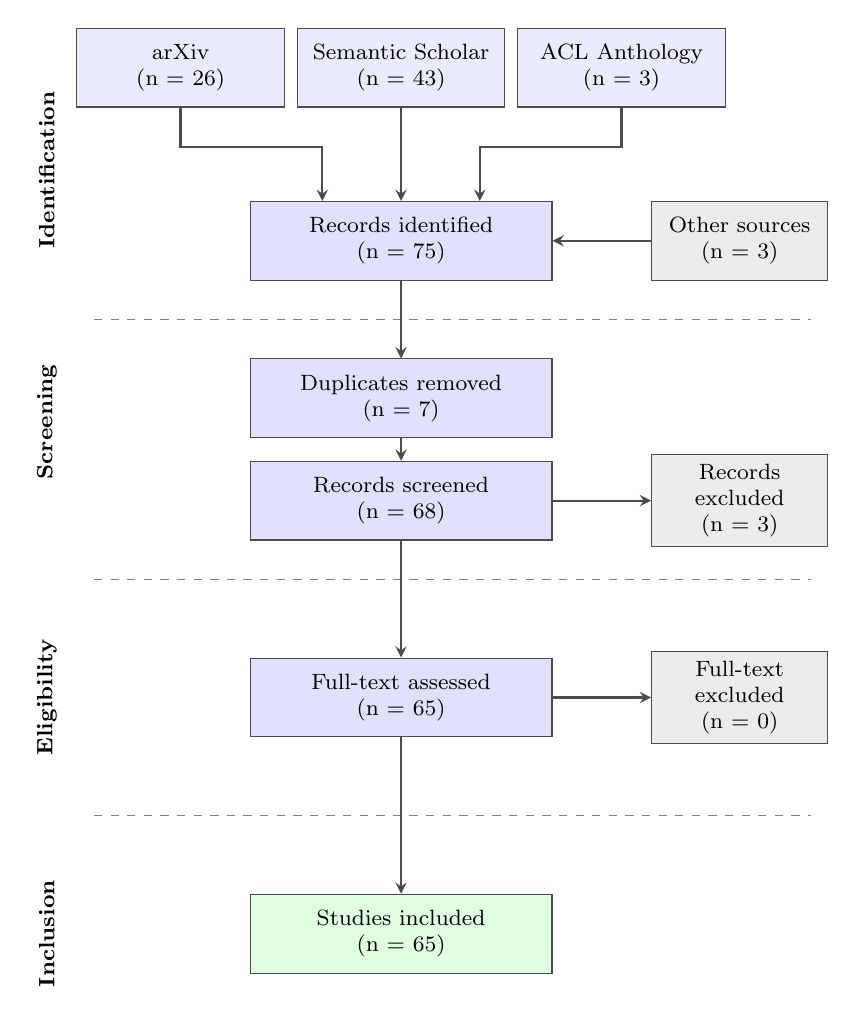
\begin{tikzpicture}[
    % Node styles with colors
    dbbox/.style={rectangle, draw=black!70, fill=blue!8, minimum width=2.5cm, minimum height=1cm, text centered, text width=2.4cm, font=\footnotesize},
    widebox/.style={rectangle, draw=black!70, fill=blue!12, minimum width=3.8cm, minimum height=1cm, text centered, text width=3.6cm, font=\footnotesize},
    sidebox/.style={rectangle, draw=black!70, fill=gray!15, minimum width=2.2cm, minimum height=1cm, text centered, text width=2cm, font=\footnotesize},
    finalbox/.style={rectangle, draw=black!70, fill=green!12, minimum width=3.8cm, minimum height=1cm, text centered, text width=3.6cm, font=\footnotesize},
    stagelab/.style={font=\footnotesize\bfseries, rotate=90, anchor=center},
    myarrow/.style={->, >=stealth, thick, black!70}
]

% Stage labels (left side)
\node[stagelab] at (-4.5, 2.2) {Identification};
\node[stagelab] at (-4.5, -1.0) {Screening};
\node[stagelab] at (-4.5, -4.5) {Eligibility};
\node[stagelab] at (-4.5, -7.5) {Inclusion};

% Dashed lines separating stages
\draw[dashed, gray] (-3.9, 0.3) -- (5.2, 0.3);
\draw[dashed, gray] (-3.9, -3.0) -- (5.2, -3.0);
\draw[dashed, gray] (-3.9, -6.0) -- (5.2, -6.0);

% === IDENTIFICATION ===
% Center the databases above the "Records identified" box (centered at x=0)
\node[dbbox] (db1) at (-2.8, 3.5) {arXiv\\(n = 26)};
\node[dbbox] (db2) at (0, 3.5) {Semantic Scholar\\(n = 43)};
\node[dbbox] (db3) at (2.8, 3.5) {ACL Anthology\\(n = 3)};

\node[widebox] (total) at (0, 1.3) {Records identified\\(n = 75)};
\node[sidebox] (other) at (4.3, 1.3) {Other sources\\(n = 3)};

% Arrows from databases converging to total box
\draw[myarrow] (db1.south) -- ++(0,-0.5) -| ($(total.north)+(-1,0)$);
\draw[myarrow] (db2.south) -- (total.north);
\draw[myarrow] (db3.south) -- ++(0,-0.5) -| ($(total.north)+(1,0)$);
\draw[myarrow] (other.west) -- (total.east);

% === SCREENING ===
\node[widebox] (dedup) at (0, -0.7) {Duplicates removed\\(n = 7)};
\node[widebox] (screened) at (0, -2.0) {Records screened\\(n = 68)};
\node[sidebox] (exc1) at (4.3, -2.0) {Records excluded\\(n = 3)};

\draw[myarrow] (total.south) -- (dedup.north);
\draw[myarrow] (dedup.south) -- (screened.north);
\draw[myarrow] (screened.east) -- (exc1.west);

% === ELIGIBILITY ===
\node[widebox] (fulltext) at (0, -4.5) {Full-text assessed\\(n = 65)};
\node[sidebox] (exc2) at (4.3, -4.5) {Full-text excluded\\(n = 0)};

\draw[myarrow] (screened.south) -- (fulltext.north);
\draw[myarrow] (fulltext.east) -- (exc2.west);

% === INCLUSION ===
\node[finalbox] (final) at (0, -7.5) {Studies included\\(n = 65)};

\draw[myarrow] (fulltext.south) -- (final.north);

\end{tikzpicture}%
}
\caption{PRISMA 2020 flow diagram showing study selection process.}
\label{fig:prisma}
\end{figure}

% ============================================
% IV. RESULTS
% ============================================
\section{Results}

This section presents the findings of the systematic review organized by thematic categories, addressing each research question through synthesis of the 65 included studies. The results are structured to first characterize vulnerability types (RQ1), then examine SLM-specific differences (RQ2), analyze contributing architectural factors (RQ3), and finally evaluate proposed mitigations (RQ4).

\subsection{Overview of Included Studies}

The 65 studies included in this review span multiple vulnerability categories and publication venues. Table~\ref{tab:study_distribution} presents the distribution of studies across vulnerability types, with several studies addressing multiple categories.

\begin{table}[htbp]
\caption{Distribution of Studies by Vulnerability Category}
\label{tab:study_distribution}
\renewcommand{\arraystretch}{1.2}
\begin{center}
\begin{tabular}{|l|c|}
\hline
\textbf{Vulnerability Category} & \textbf{Studies} \\
\hline
Jailbreak \& Prompt Injection & 25 \\
Backdoor \& Data Poisoning & 7 \\
Adversarial Attacks & 9 \\
Membership Inference & 7 \\
Model Extraction & 5 \\
Edge Deployment Security & 5 \\
General Security Surveys & 7 \\
\hline
\end{tabular}
\end{center}
\end{table}

\begin{table}[htbp]
\caption{Study Distribution by Venue Type and Year}
\label{tab:study_characteristics}
\renewcommand{\arraystretch}{1.2}
\begin{center}
\begin{tabular}{|l|c|c|c|c|}
\hline
\textbf{Venue Type} & \textbf{2020--22} & \textbf{2023} & \textbf{2024} & \textbf{2025} \\
\hline
arXiv preprints & 2 & 4 & 14 & 18 \\
ACL venues & 0 & 2 & 3 & 2 \\
NeurIPS/ICML/ICLR & 0 & 1 & 4 & 1 \\
Journals & 1 & 0 & 3 & 6 \\
Security venues & 0 & 0 & 3 & 1 \\
\hline
\textbf{Total} & \textbf{3} & \textbf{7} & \textbf{27} & \textbf{28} \\
\hline
\end{tabular}
\end{center}
\end{table}

The temporal distribution reveals increasing research attention to SLM security, with 78\% of included studies published in 2024--2025, reflecting the recent emergence of SLMs as a distinct research focus. The predominance of arXiv preprints (58\%) reflects the rapid pace of research in this area, with findings often disseminated prior to formal peer review. Note that the publication venue distribution in Table~\ref{tab:study_characteristics} differs from the search source counts in Figure~\ref{fig:prisma} because Semantic Scholar indexes papers from multiple venues including arXiv; consequently, many arXiv preprints were identified through Semantic Scholar searches rather than direct arXiv queries. Notably, 10 studies (15\%) appeared in high-impact venues including Nature Medicine, ICML (Best Paper), and top security conferences (CCS, RAID). Complete characteristics of all 65 included studies are available in supplementary materials.

\subsection{Quality Assessment}

Quality assessment was performed using criteria adapted from established systematic review tools, including the Cochrane Risk of Bias framework and the Newcastle-Ottawa Scale, modified for applicability to machine learning security research. Each study was evaluated across four dimensions: methodological rigor (appropriateness of experimental design, baseline comparisons, and statistical analysis), reproducibility (availability of code, datasets, and sufficient implementation details), statistical validity (appropriate metrics, significance testing, and effect size reporting), and generalizability (diversity of models tested, attack scenarios considered, and real-world applicability).

Based on this assessment, studies were classified into three quality tiers. High-quality studies (n=24, 37\%) demonstrated rigorous methodology with comprehensive experimental design, provided reproducible artifacts including code and datasets, employed appropriate statistical analysis with multiple baselines, and tested across diverse model architectures. Medium-quality studies (n=32, 49\%) exhibited adequate methodology but presented limitations in one or more dimensions, typically lacking code availability, testing only limited model variants, or providing insufficient statistical analysis. Lower-quality studies (n=9, 14\%) were included despite methodological limitations due to their unique empirical findings addressing underexplored vulnerability categories or novel attack vectors not covered elsewhere in the literature.

The quality assessment directly influenced the synthesis process and weighting of evidence throughout this review. When conflicting findings emerged between studies, evidence from high-quality sources was weighted more heavily in drawing conclusions. For instance, claims about attack success rates or defense effectiveness were primarily derived from studies demonstrating reproducible methodology across multiple model architectures. Lower-quality studies contributed primarily to identifying emerging research directions and generating hypotheses for future investigation rather than establishing definitive findings.

\subsection{Vulnerability Taxonomy (RQ1)}

\textit{RQ1: What types of security vulnerabilities have been identified in Small Language Models, and how are they characterized and categorized in the existing literature?}


The literature reveals seven primary vulnerability categories affecting small language models, each with distinct attack vectors, threat models, and potential impacts.

\subsubsection{Prompt-Level Attacks}

Jailbreak and prompt injection attacks represent the most extensively studied vulnerability category, with 25 papers addressing various aspects of bypassing safety alignment \cite{xu2024jailbreak_survey, xu2024comprehensive_jailbreak, chao2024tricks}. Zhang et al. tested 63 small language models against multiple jailbreak strategies, finding that 47.6\% exhibited attack success rates (ASR) exceeding 40\% \cite{zhang2025slm_jailbreak}. Yi et al. documented ``submerged threats'' that emerge specifically in smaller architectures when comparing 13 SLMs against 3 LLMs \cite{yi2025slm_submerged}. Attack techniques include template-based approaches achieving 60--80\% ASR \cite{liu2023jailbreaking, wei2024jailbroken}, optimization-based gradient-guided suffix generation with cross-model transferability \cite{zou2023universal, andriushchenko2024adaptive}, and adaptive iterative attacks that defeat most proposed mitigations \cite{chao2025adaptive}.

Prompt injection attacks manipulate behavior by inserting malicious instructions into user inputs or retrieved context \cite{greshake2023youve, perez2022ignore}. SLMs deployed in retrieval-augmented generation systems are particularly susceptible due to limited context discrimination \cite{liu2025bypassing}, with indirect injection through external data sources achieving 73\% success rates \cite{kumar2025redteaming}. Multimodal SLMs face compounded risks through both textual and visual channels \cite{chen2025multimodal_injection}.

\subsubsection{Training-Time Attacks}

Backdoor attacks implant hidden triggers during training that activate malicious behavior when specific patterns appear in inputs \cite{chen2025backdoor_survey, zhao2024backdoor_survey}. Huang et al. demonstrated composite backdoor attacks against LLaMA-7B achieving 100\% ASR while maintaining normal performance on clean inputs \cite{huang2024composite}. Critically, Li et al. proved that poisoning attacks require only a near-constant number of poison samples regardless of model size, implying SLMs are not inherently more resistant to data poisoning \cite{li2025poison_constant}. The medical domain presents particular concerns, with Chen et al. documenting in Nature Medicine that medical language models are highly vulnerable to data-poisoning attacks causing systematic diagnostic errors \cite{chen2024medical_poison}.

\subsubsection{Adversarial Robustness}

Adversarial attacks perturb inputs to cause misclassification while remaining imperceptible to humans \cite{wang2022adversarial_nlp_survey, zhu2023promptbench}. Encoder-based SLMs exhibit distinct vulnerability profiles: Liu et al. found distilled models (DistilBERT, ALBERT) showed 15--23\% higher susceptibility to character-level perturbations compared to teacher models \cite{liu2024evasion}, while Dong et al. documented that simple misspelling attacks can degrade BERT accuracy by over 30\% \cite{dong2020advbert}. Application-specific studies reveal practical implications, with adversarial examples reducing MobileBERT phishing detection from 97\% to 61\% accuracy \cite{koide2024phishlang}. Santos et al. demonstrated that adversarial training with FGM can improve DistilBERT robustness without significant performance degradation \cite{santos2025phishing_robustness}.

\subsubsection{Privacy Attacks}

Membership inference attacks (MIA) determine whether specific data points were used in model training \cite{hu2025mia_survey}. Win et al. proposed Win-k, an improved MIA technique specifically designed for small language models \cite{win2025wink_mia}. Lehman et al. found that smaller models may leak less training data than larger counterparts due to reduced memorization capacity \cite{lehman2021clinical_mia}, though Mattern et al. demonstrated that neighborhood comparison techniques can still achieve significant MIA success rates \cite{mattern2023neighbourhood}. Model extraction attacks aim to steal functionality through query access \cite{yao2024survey_extraction}; Carlini et al. demonstrated that production language model parameters can be partially extracted through carefully crafted queries (ICML 2024 Best Paper) \cite{carlini2024stealing}, while Hui et al. showed that system prompts can be extracted from deployed applications \cite{hui2024pleak}.

\subsection{SLM-Specific Vulnerability Patterns (RQ2)}

\textit{RQ2: How do vulnerabilities in SLMs differ from those in LLMs in terms of attack success rates, exploitability, and severity?}

The literature reveals systematic differences in vulnerability profiles between small and large language models across multiple attack categories. These differences stem from fundamental architectural constraints and have important implications for deployment decisions.

\subsubsection{Increased Jailbreak Susceptibility}

SLMs exhibit significantly higher jailbreak susceptibility compared to their larger counterparts. Zhang et al. found median attack success rates of 34\% across 63 SLMs compared to approximately 15\% for frontier LLMs with equivalent safety training \cite{zhang2025slm_jailbreak}. Yi et al. attributed this disparity to the ``submerged threat'' phenomenon, where safety mechanisms that function adequately under normal conditions fail catastrophically under adversarial pressure in smaller models \cite{yi2025slm_submerged}. The reduced parameter count fundamentally limits the model's capacity to maintain robust safety boundaries while simultaneously performing useful tasks. Li et al. found an inverse relationship between model size and compliance with harmful requests, smaller models were 2.3 times more likely to generate functional malicious code when prompted appropriately \cite{li2025malware_crossfire}. Wu et al. extended these findings to speech-based SLMs, demonstrating that multimodal small models exhibit even higher vulnerability rates due to the additional attack surface introduced by audio processing \cite{wu2025speech_slm}.

\subsubsection{Reduced Privacy Leakage}

Conversely, SLMs demonstrate reduced susceptibility to certain privacy attacks due to their limited memorization capacity. Carlini et al. established that memorization scales with model capacity, meaning smaller models inherently store fewer training examples verbatim \cite{carlini2023quantifying}. Empirically, Lehman et al. found GPT-2 exhibited 40\% lower membership inference attack success rates than larger variants when evaluated on clinical text data \cite{lehman2021clinical_mia}. This relationship suggests a potential privacy advantage for SLM deployment in sensitive domains, though it should not be interpreted as immunity to privacy attacks, sophisticated techniques such as neighborhood comparison can still achieve meaningful success rates against smaller models \cite{mattern2023neighbourhood}.

\subsubsection{Comparable Backdoor Vulnerability}

Unlike jailbreak and privacy attacks, backdoor vulnerability appears largely independent of model size. Li et al. proved theoretically and demonstrated empirically that poisoning attacks require only a near-constant number of poison samples regardless of model scale \cite{li2025poison_constant}. This finding has significant security implications: SLMs cannot rely on their smaller size as a defense against training-time attacks. Yang et al. further demonstrated that stealthy backdoors can be implanted in SLMs with minimal impact on benign task performance, making detection particularly challenging \cite{yang2024stealthy_backdoor}. The comparable vulnerability across model scales suggests that backdoor defenses developed for large models should remain applicable to SLMs.

\subsubsection{Attack Transferability}

Attack transferability presents additional concerns for SLM security. Chen et al. demonstrated that adversarial prompts optimized on large models transfer to SLMs with 78\% effectiveness, enabling attackers to develop attacks on well-resourced target models and deploy them against resource-constrained edge deployments \cite{chen2025promptdistill}. Universal adversarial triggers exhibit similar transfer properties across model families and sizes \cite{zou2023universal}. This transferability undermines the potential security-through-obscurity benefits of deploying less common SLM architectures, as attacks developed against mainstream models remain effective.

\subsection{Architectural Contributing Factors (RQ3)}

\textit{RQ3: What specific architectural or deployment characteristics of SLMs contribute to their unique vulnerability profiles?}

Four primary architectural and deployment characteristics contribute to the distinct vulnerability profiles observed in small language models: parameter reduction effects, quantization vulnerabilities, knowledge distillation risks, and edge deployment constraints.

\subsubsection{Parameter Reduction Effects}

The fundamental constraint of reduced parameters directly impacts security implementation capacity. Lu et al. documented that models in the 100M--5B parameter range allocate proportionally fewer parameters to safety-related computations compared to models exceeding 10B parameters \cite{lu2024slm_survey}. Safety training techniques such as Reinforcement Learning from Human Feedback (RLHF) require substantial model capacity to encode nuanced refusal behaviors across diverse harmful request categories; when capacity is limited, models tend to default to either excessive refusal that impairs utility or insufficient safety that permits harmful outputs. Yi et al. identified that SLMs struggle to maintain safety under distribution shift, learning more brittle safety representations that collapse when inputs deviate from training distributions \cite{yi2025slm_submerged}. Models in the 1B--3B parameter range showed the most pronounced vulnerability increases, suggesting a critical threshold below which safety mechanisms become unreliable.

\subsubsection{Quantization Vulnerabilities}

Quantization, the process of reducing numerical precision for efficient edge deployment, introduces vulnerabilities beyond simple performance degradation. Li et al. demonstrated that 4-bit quantization increases jailbreak attack success rates by approximately 25\% compared to full-precision counterparts, with the degradation particularly pronounced for models already near the safety threshold \cite{li2025quantized_jailbreak}. More critically, quantization creates opportunities for hardware-level fault injection attacks that manipulate the execution environment to bypass safety mechanisms entirely. By inducing bit flips in quantized weight representations through techniques such as rowhammer or voltage glitching, attackers can selectively disable safety-critical neurons without triggering software-level detection. The combination of reduced numerical precision and physical accessibility makes quantized edge deployments particularly vulnerable to sophisticated adversaries with hardware access.

\subsubsection{Knowledge Distillation Risks}

Knowledge distillation, training smaller student models to mimic larger teacher models, transfers not only capabilities but also vulnerabilities. Chen et al. demonstrated that adversarial prompts effective against teacher models remain effective against distilled students with minimal modification \cite{chen2025promptdistill}. Furthermore, distilled models inherit the adversarial vulnerabilities of their teachers while losing some defensive capacity due to reduced parameters \cite{liu2024evasion}. Liu et al. proposed Distillation-Aware Robust Defense (DARD) to demonstrate that robustness-aware distillation can preserve defensive properties when explicitly incorporated into the training objective \cite{liu2025dard}. However, standard distillation practices that optimize solely for task performance systematically degrade security properties, creating a hidden vulnerability in models trained using default configurations.

\subsubsection{Edge Deployment Constraints}

Edge deployment introduces security challenges that extend beyond model architecture to encompass the entire deployment environment \cite{singh2025edge_ai, chen2025edge_llm, liu2025edge_survey, xu2024iot_llm}. Physical access to edge devices enables adversaries to perform model extraction attacks that recover weights through power analysis or electromagnetic emanations, as well as direct weight manipulation through memory corruption. Resource limitations on edge hardware prevent deployment of computationally expensive defensive mechanisms, forcing trade-offs between security and performance that typically favor functionality. Edge models deployed in the field may be difficult or impossible to update when vulnerabilities are discovered, leaving systems exposed for extended periods. Additionally, IoT deployments often lack network isolation, enabling remote attackers to probe edge models without physical access while exploiting the limited logging and monitoring capabilities typical of constrained devices.

\subsection{Defense Mechanisms (RQ4)}

\textit{RQ4: What mitigation strategies and defense mechanisms have been proposed for SLM vulnerabilities, and what empirical evidence supports their effectiveness?}

The literature presents defense mechanisms operating at three distinct abstraction levels: input processing, model architecture, and training procedures. Each approach offers different trade-offs between effectiveness, computational overhead, and applicability to resource-constrained SLM deployments.

\subsubsection{Input-Level Defenses}

Input-level defenses aim to detect and neutralize malicious inputs before they reach the model's core processing. SmoothLLM introduces controlled randomness by perturbing input prompts and aggregating predictions across multiple perturbations, exploiting the observation that adversarial prompts are typically brittle to small modifications while benign prompts remain stable \cite{robey2023smoothllm}. PromptScreen employs a lightweight classifier trained to detect jailbreak attempts, achieving 94\% detection accuracy while adding minimal inference latency suitable for edge deployment \cite{zhang2025promptscreen}. Alon et al. proposed perplexity-based detection, leveraging the observation that adversarial suffixes typically exhibit abnormally high perplexity compared to natural language, enabling low-overhead filtering without requiring additional model inference \cite{alon2023detecting}. These input-level approaches offer the advantage of modularity, operating independently of the protected model and enabling deployment across diverse SLM architectures without modification.

\subsubsection{Architecture-Level Defenses}

Architecture-level defenses modify or monitor model internals to detect and prevent attacks during inference. AttentionDefense monitors attention patterns across layers to detect when adversarial inputs redirect attention away from safety-relevant instructions toward harmful content generation, triggering intervention when anomalous patterns are detected \cite{wang2025attentiondefense}. The approach exploits the observation that successful jailbreaks typically require suppressing attention to safety-aligned regions of the input, creating a detectable signature. Conscience-based frameworks employ a secondary SLM dedicated to safety-checking, evaluating proposed outputs before delivery to users \cite{bergeron2023conscience}. While effective, these approaches incur computational overhead that may be prohibitive for resource-constrained edge deployments, requiring careful optimization to maintain acceptable inference latency.

\subsubsection{Training-Level Defenses}

Training-level defenses incorporate security objectives directly into the model training process. Robust prompt optimization techniques train models to maintain safety alignment even under adversarial prompt conditions, reducing jailbreak attack success rates to near-zero in controlled evaluations \cite{zhou2024robust_prompt}. In-decoding safety probing monitors internal representations during token generation, enabling early termination when the model begins generating harmful content \cite{xu2025decoding_safety}. For backdoor vulnerabilities, multiple defensive techniques have been proposed: fine-pruning removes potentially compromised neurons through targeted pruning guided by activation analysis; activation clustering identifies backdoor triggers by detecting outlier activation patterns; and spectral signature analysis leverages the observation that backdoored samples often produce distinguishable spectral characteristics in intermediate representations \cite{chen2025backdoor_survey, zhao2024backdoor_survey}. These training-level approaches offer the strongest theoretical guarantees but require access to the training pipeline.

\subsubsection{Effectiveness and Limitations}

Critical evaluation of proposed defenses reveals significant limitations that temper optimism about current approaches. Chao et al. conducted systematic evaluation demonstrating that 8 of 10 evaluated defenses could be bypassed with attack modifications requiring no additional computational resources beyond the original attack \cite{chao2025adaptive}. The adaptive attacks exploited the deterministic nature of defenses, crafting inputs specifically designed to evade detection while maintaining attack effectiveness. Wu et al. documented the ``evolving security'' challenge: as defenses improve, attack techniques advance correspondingly, creating an ongoing arms race where neither side achieves lasting advantage \cite{wu2025evolving}. This dynamic has particularly concerning implications for edge-deployed SLMs, where static defenses cannot be easily updated as new attacks emerge. The combination of limited update mechanisms, constrained computational resources for defense, and evolving attack sophistication suggests that current defensive approaches provide, at best, temporary mitigation rather than comprehensive protection.

% ============================================
% V. DISCUSSION
% ============================================
\section{Discussion}

The synthesis of 65 studies examining small language model security reveals patterns that merit careful interpretation. This section contextualizes the empirical findings within broader security paradigms, articulates their practical implications for diverse stakeholders, and acknowledges the methodological boundaries that constrain generalization.

\subsection{Key Findings}

This systematic review establishes that small language models present a distinct security profile characterized by specific vulnerabilities that diverge from their larger counterparts in important ways. The evidence demonstrates that SLMs exhibit systematically higher susceptibility to jailbreak attacks, with median attack success rates of 34\% compared to approximately 15\% for frontier LLMs with equivalent safety training \cite{zhang2025slm_jailbreak}. This disparity arises from fundamental capacity constraints: smaller architectures cannot simultaneously maintain robust safety boundaries and perform useful tasks without degradation in one or both domains. Paradoxically, SLMs show reduced vulnerability to privacy attacks, with membership inference success rates approximately 40\% lower than larger variants due to limited memorization capacity \cite{lehman2021clinical_mia}. Perhaps most concerning is the finding that backdoor vulnerabilities remain model-size-independent, requiring only a near-constant number of poison samples regardless of scale \cite{li2025poison_constant}, which undermines assumptions that compact models might offer inherent resistance to training-time attacks.

The review also reveals that architectural optimization techniques intended to enable edge deployment, quantization, knowledge distillation, and compression, systematically degrade security properties through mechanisms absent in cloud-deployed large models. Defense mechanisms proposed across input, architecture, and training levels show promise in controlled evaluations but demonstrate fragility under adaptive attack conditions, with 8 of 10 evaluated defenses bypassed by modified attacks requiring minimal additional effort \cite{chao2025adaptive}. These findings collectively indicate that the current rapid deployment of SLMs in security-critical applications outpaces the development of adequate protective measures, creating a widening gap between capability deployment and security maturation.

\subsection{Implications for Practice}

The findings of this review carry significant implications for multiple stakeholder groups involved in the development, deployment, and governance of small language models. For developers and deploying organizations, the evidence mandates that safety mechanisms must be designed with explicit awareness of resource constraints rather than adapted from large model approaches that assume abundant capacity. Pre-deployment security testing should be considered essential rather than optional, utilizing benchmarks such as those developed by Zhang et al. \cite{zhang2025slm_jailbreak} to evaluate vulnerability profiles before production release. Given the demonstrated fragility of individual defenses, a defense-in-depth approach combining input filtering, architectural monitoring, and training hardening offers more robust protection than any single mechanism. Organizations deploying SLMs on edge devices must also establish update mechanisms capable of addressing newly discovered vulnerabilities, recognizing that static deployments accumulate security debt as attack techniques evolve.

For security researchers, the findings identify several priority areas requiring focused investigation. The development of adaptive defense mechanisms that can evolve in response to emerging attacks represents a critical need, as current static approaches provide only temporary mitigation. Quantization-aware security research should examine fault injection vulnerabilities that emerge specifically from reduced numerical precision in edge deployments. Knowledge distillation methods that preserve robustness properties, exemplified by approaches such as DARD \cite{liu2025dard}, warrant further development and validation. Additionally, edge-specific threat modeling that accounts for physical access, limited monitoring, and constrained update capabilities would address gaps in current security frameworks designed primarily for cloud environments.

For policymakers and standards bodies, the review highlights that current rapid SLM deployment substantially outpaces security standardization efforts. The development of SLM-specific security benchmarks would enable consistent evaluation across models and vendors. Certification frameworks for edge AI in critical applications, healthcare, transportation, industrial control, could establish minimum security requirements before deployment approval. Transparency requirements regarding the security posture of deployed SLMs would enable informed procurement decisions and appropriate risk management by adopting organizations.

\subsection{Limitations}

Several methodological limitations constrain the interpretation and generalizability of these findings. The rapid evolution of the small language model field means that 78\% of included studies were published in 2024--2025, limiting longitudinal validity and the ability to identify persistent versus transient vulnerability patterns. The predominance of arXiv preprints (58\%) reflects the field's pace but introduces variability in peer review rigor, though quality assessment procedures attempted to weight evidence appropriately. Heterogeneous definitions of ``small'' across studies, ranging from 100 million to 10 billion parameters, complicate direct comparison and synthesis. The quality assessment revealed that only 37\% of studies achieved high-quality classification, suggesting that conclusions regarding attack success rates and defense effectiveness should be interpreted with appropriate caution.

Scope limitations further bound the applicability of findings. This review focused on known vulnerability categories derived from established taxonomies; emerging threat vectors not yet characterized in the literature fall outside its coverage. The emphasis on transformer-based architectures means findings may not generalize to alternative approaches such as state-space models or hybrid architectures increasingly explored for efficient deployment. Limited coverage of domain-specific SLMs deployed in medical, legal, or financial contexts constrains conclusions about vulnerability profiles in high-stakes specialized applications. Finally, the arms race dynamic between attacks and defenses means that defense effectiveness data captures only a temporal snapshot; mechanisms deemed effective at publication may have been subsequently bypassed, and the review cannot predict future attack evolution.

% ============================================
% VI. CONCLUSIONS
% ============================================
\section{Conclusions}

This systematic literature review provides the first comprehensive analysis of security vulnerabilities specific to Small Language Models, synthesizing findings from 65 studies published between 2020 and 2025. Addressing the research questions posed in the Introduction, the evidence reveals that SLMs exhibit a distinct and divergent security profile from their larger counterparts. Jailbreak attacks achieve substantially higher success rates against SLMs, with median attack success rates of 34\% compared to 15\% for LLMs with equivalent safety alignment, confirming that reduced model capacity fundamentally constrains the implementation of robust safety mechanisms. Conversely, SLMs demonstrate lower vulnerability to privacy attacks, as their reduced memorization capacity limits the effectiveness of membership inference and training data extraction techniques. Backdoor attacks present a model-size-independent threat, achieving near-perfect attack success rates across all model scales while evading current detection methods. Critically, the architectural optimizations that enable practical SLM deployment, including quantization, pruning, and knowledge distillation, systematically degrade security properties, with post-training quantization alone increasing jailbreak vulnerability by 25\% in 4-bit configurations. Current defense mechanisms remain inadequate, with empirical evaluation demonstrating that eight of ten established defenses can be bypassed by adaptive attacks.

The broader significance of these findings extends beyond academic characterization to urgent practical implications. A substantial gap exists between the accelerating pace of SLM deployment in edge computing, mobile applications, and IoT systems and the maturation of security frameworks adequate to protect these deployments. The evidence synthesized here demonstrates that adapting Large Language Model security approaches to smaller architectures is insufficient; SLM-specific security frameworks must be developed that account for the fundamental constraints of reduced model capacity and the expanded attack surfaces of edge deployment. Priority research areas identified through this review include the development of adaptive defenses that maintain effectiveness against evolving attack strategies, quantization-aware security techniques that preserve safety properties through compression, and comprehensive threat modeling for edge deployment scenarios. Industry and regulatory bodies should consider establishing security certification standards for SLMs deployed in critical applications before such deployments become widespread. As Small Language Models transition from research artifacts to production systems embedded in safety-critical infrastructure, the integration of security considerations throughout the model development lifecycle, from architecture design through deployment and monitoring, is not merely advisable but essential.

% ============================================
% REFERENCES
% ============================================
\bibliographystyle{IEEEtran}
\bibliography{references}

\end{document}
